\presec
\section{Experimental Results} \postsec
\label{sec:evaluation}
%The goal of this section is to validate the accuracy and correctness of our proposed bound and formula.
In this section, we first validate our proposed formula of optimal $k$ (Eq. \ref{equ:mykform}).
Second, we compare our proposed upper bound of the FP probability of BFs (Eq. \ref{bounds}) with Bose's upper bound (Eq. \ref{fBound}). 
Third, we validate our proposed upper and lower bounds of the correct rate of CBFs (Eq. \ref{cbfbounds}). 

\presub
\subsection{Experimental Setup}\postsub
\label{setup}

\noindent\textbf{Datasets: }
%\para{}
We use the anonymized IP trace collected in 2016 from CAIDA \cite{caida}.
Each flow is identified by its source IP address (sip) and destination IP address (dip). 
For BF, each distinct sip-dip pair from this trace functions as an element in the aforementioned set. 
We use (part of) the first 100M distinct sip-dip pairs to construct BFs, and query the next 300M distinct sip-dip pairs to get the empirical FP probabilities of these BFs. 
For CBF, each distinct sip-dip pair and its occurrence number from this trace function as a distinct element and the corresponding frequency in the aforementioned multiset, respectively. 
We use (part of) the first 100M distinct sip-dip pairs and their occurrence numbers in the current trace to construct CBFs, and query their frequencies to get the empirical correct rates of these CBFs. 

\noindent\textbf{Implementation: }
We have implemented the standard Bloom filter in C\texttt{++}.
We use the Bob Hash (obtained from the open source website \cite{bobhash}) with different initial seeds to implement the hash functions in BFs as recommended by literature \cite{hashformeasure}. 
All the implementation source code is made publicly available anonymously at GitHub \cite{opensource}.

%\noindent\textbf{Computation Platform: }
%We performed all the experiments on a machine with 12-core CPUs (24 threads, Intel Xeon CPU E5-2620 @2 GHz) and 62 GB total DRAM memory.
%Each CPU core has three levels of cache memory: two 32KB L1 caches (one is a data cache and the other is an instruction cache) for each core, one 256KB L2 cache for each core, and one 15MB L3 cache shared by all cores.

\subsection{Optimal $k$ Formula Validation}

\subsubsection{Optimal $k$ vs. $n$}
Figure \ref{opt_k_n} plots the empirically and theoretically optimal $k$ with different $n$ increasing from 10M to 100M with a step of 10M for $m = 500$M. 
\textit{Our results show that the optimal $k$ calculated from our new formula follows the empirically optimal $k$ very well, regardless of the values of $n$.} 
We observe that the optimal $k$ calculated from our new formula is very close to the one calculated from the formula obtained by Bloom. 
The reason is that the above two formulas about the optimal $k$ have the same asymptotic form when $m$ is large enough (see Section \ref{optk}). 


\begin{figure}[t]
	\centering
	\prefig
	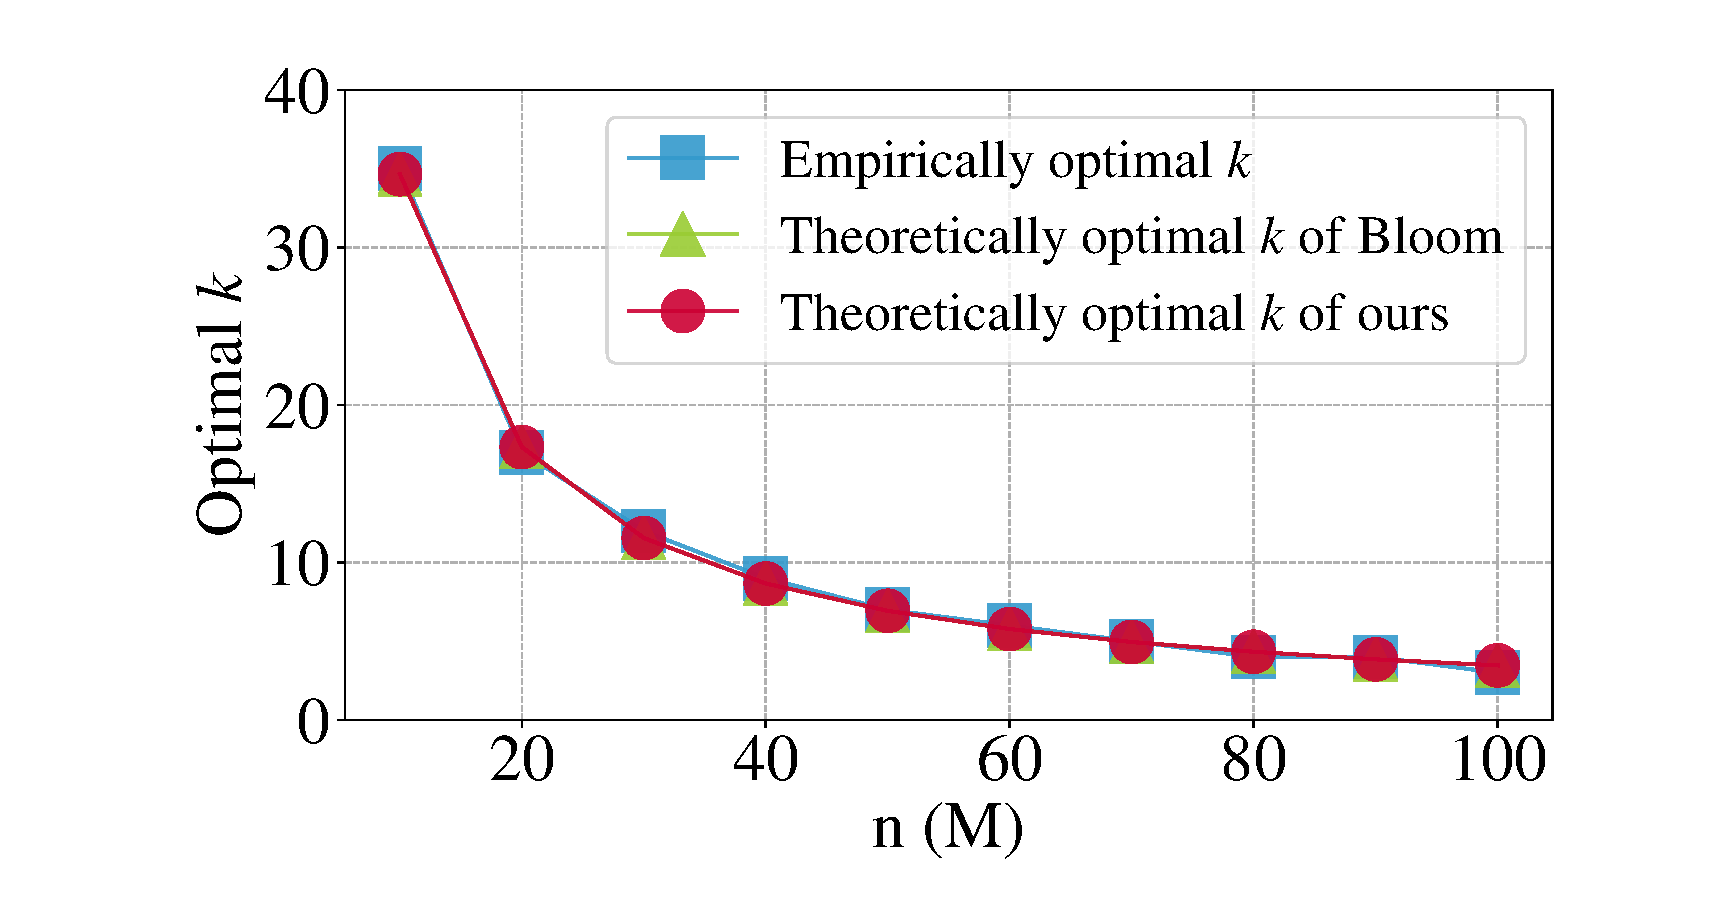
\includegraphics[width=0.288\textwidth]{opt_k_n}
	\postfig
	\precaption\adjustfigs
	\caption{Optimal $k$ vs. $n$ for $m = 500$M.}
	\postcaption
	\label{opt_k_n}
	\vspace{0.05in}
\end{figure}


\subsubsection{Optimal $k$ vs. $m$}

Figure \ref{opt_k_m} plots the empirically and theoretically optimal $k$ with different $m$ increasing from 100M to 1000M with a step of 100M for $n = 50$M. 
\textit{Our results show that the optimal $k$ calculated from our new formula follows the empirically optimal $k$ very well, regardless of the values of $m$.} 
We observe that the optimal $k$ calculated from our new formula is very close to the one calculated from the formula obtained by Bloom, especially when $m$ becomes larger. 
%The reason is that the above two formulas about the optimal $k$ have the same asymptotic form when $m$ is large enough (see Section \ref{optk}). 

\begin{figure}[t]
	\centering
	\prefig
	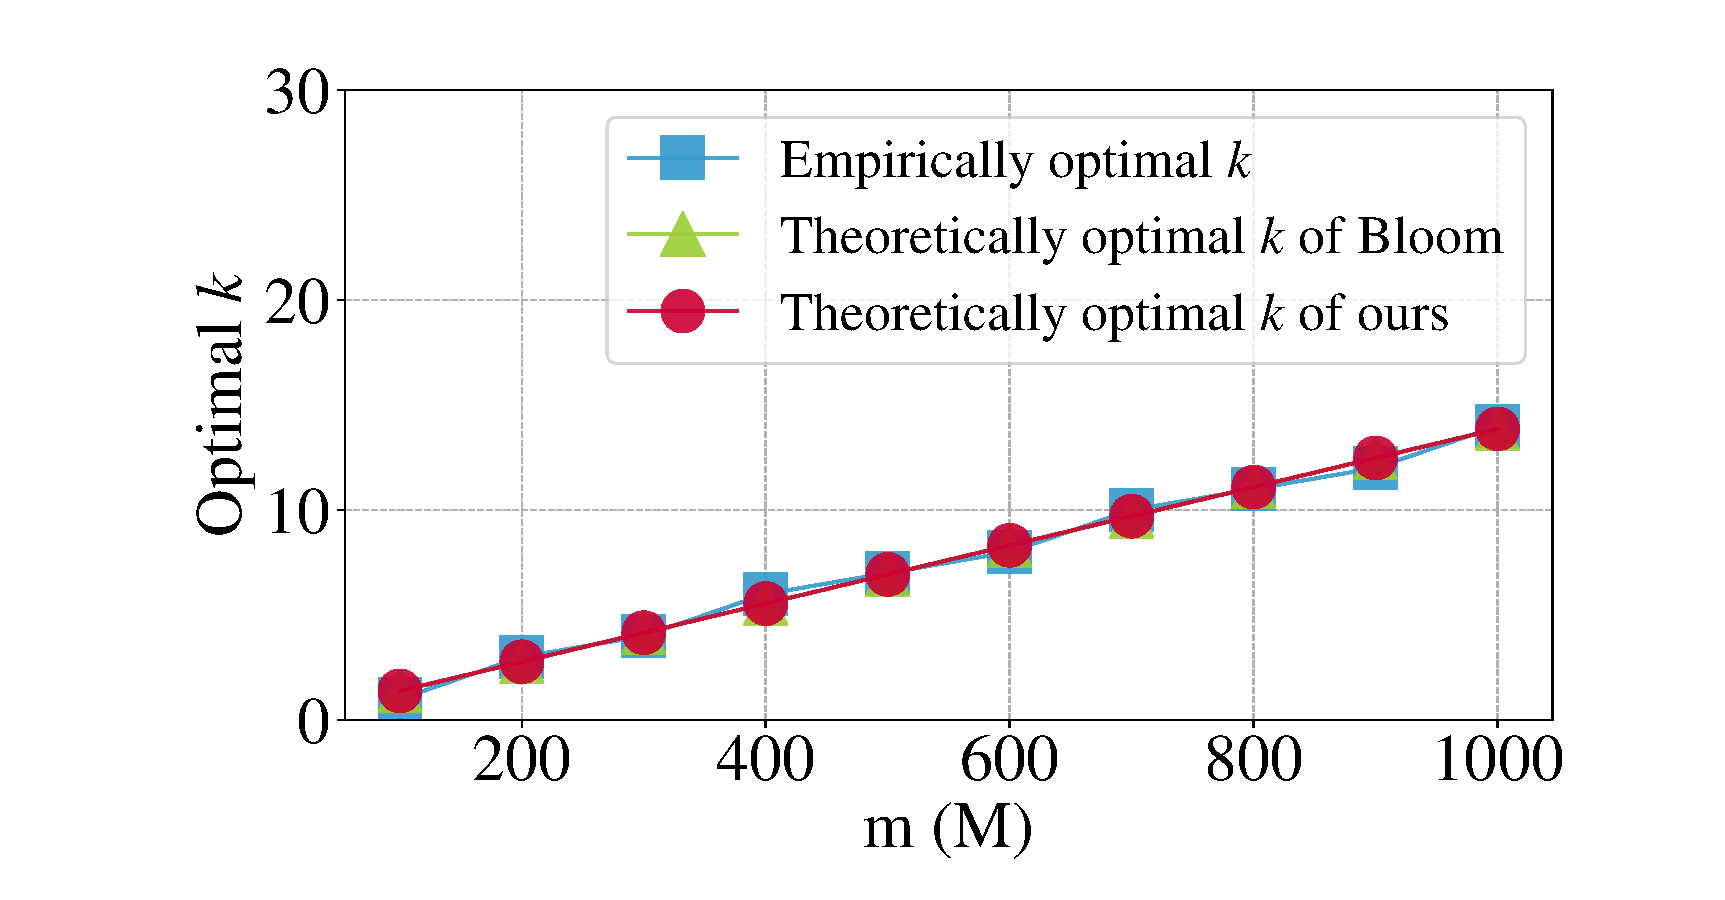
\includegraphics[width=0.288\textwidth]{opt_k_m}
	\postfig \precaption
	\adjustfigs
	\caption{Optimal $k$ vs. $m$ for $n = 50$M.}
	\label{opt_k_m}
	\postcaption
\end{figure}



%\vspace{-0.1in}
\subsection{Upper Bound Comparison}


\begin{figure*}[t!]
	\vspace{0.1in}
	\centering
	%
	\begin{minipage}[t]{0.32\textwidth}{
			\prefig
			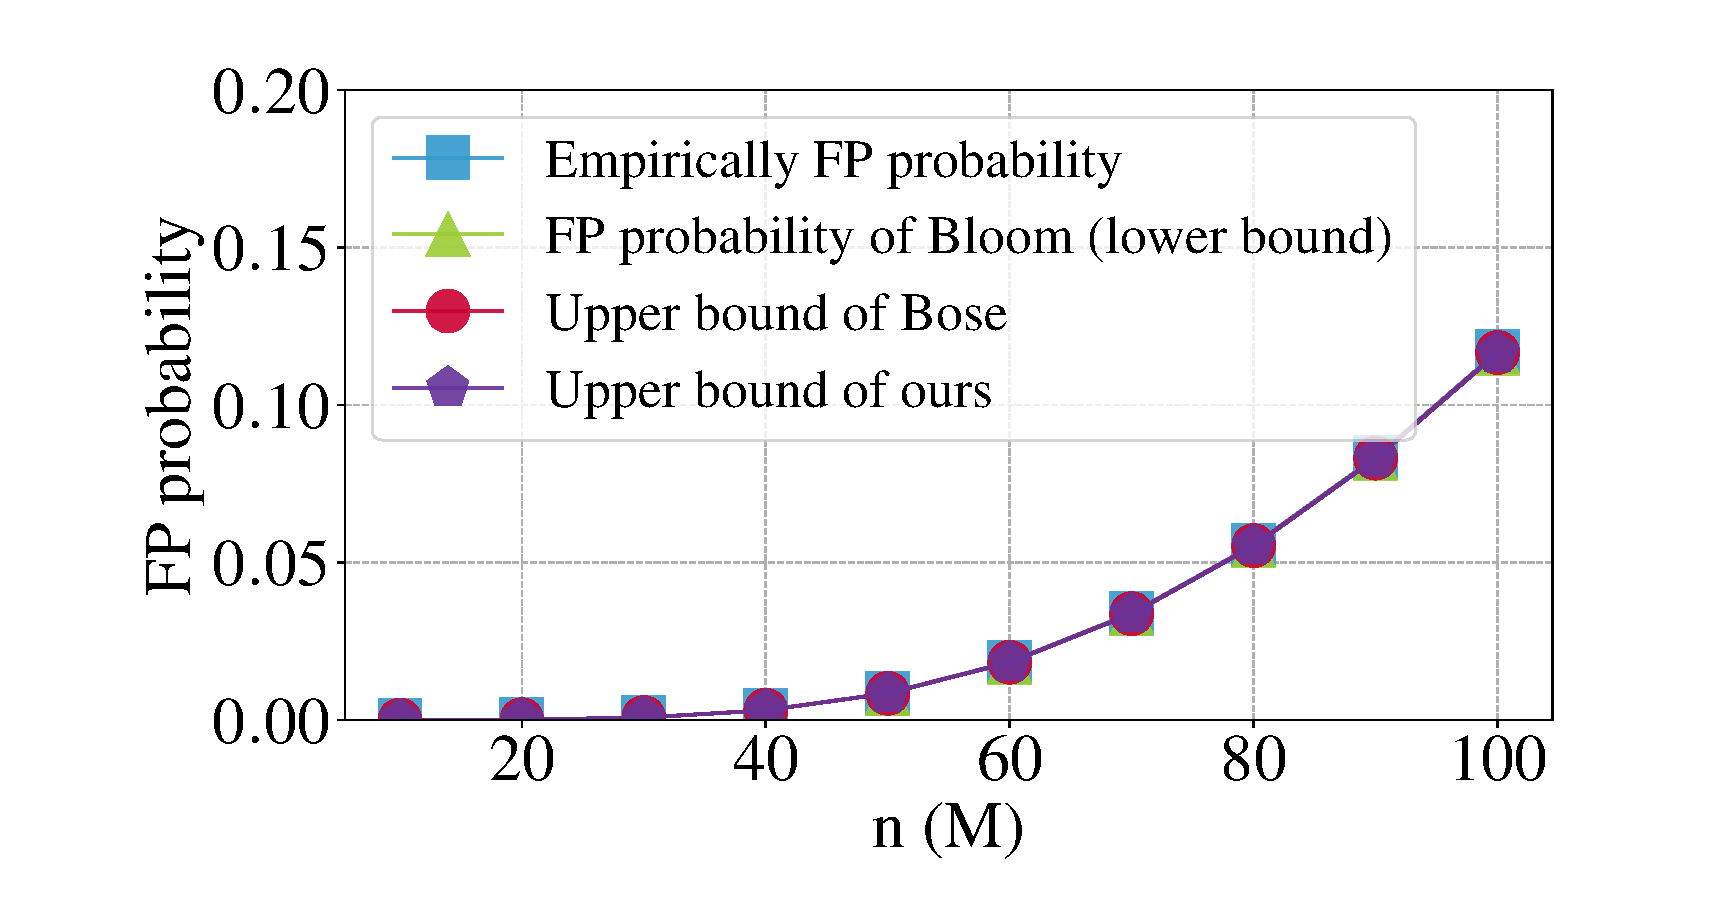
\includegraphics[width=0.90\textwidth, height=1.125in]{upbound_n}}
		\postfig\precaption\adjustfigs
%		\vspace{-0.05in}
		\caption{FP probability vs. $n$ for $m = 500$M and $k = 6$.}
		\label{upbound_n}\postcaption
	\end{minipage}
	%
	\begin{minipage}[t]{0.32\textwidth}{
			\prefig
			\vspace{0.02in}
			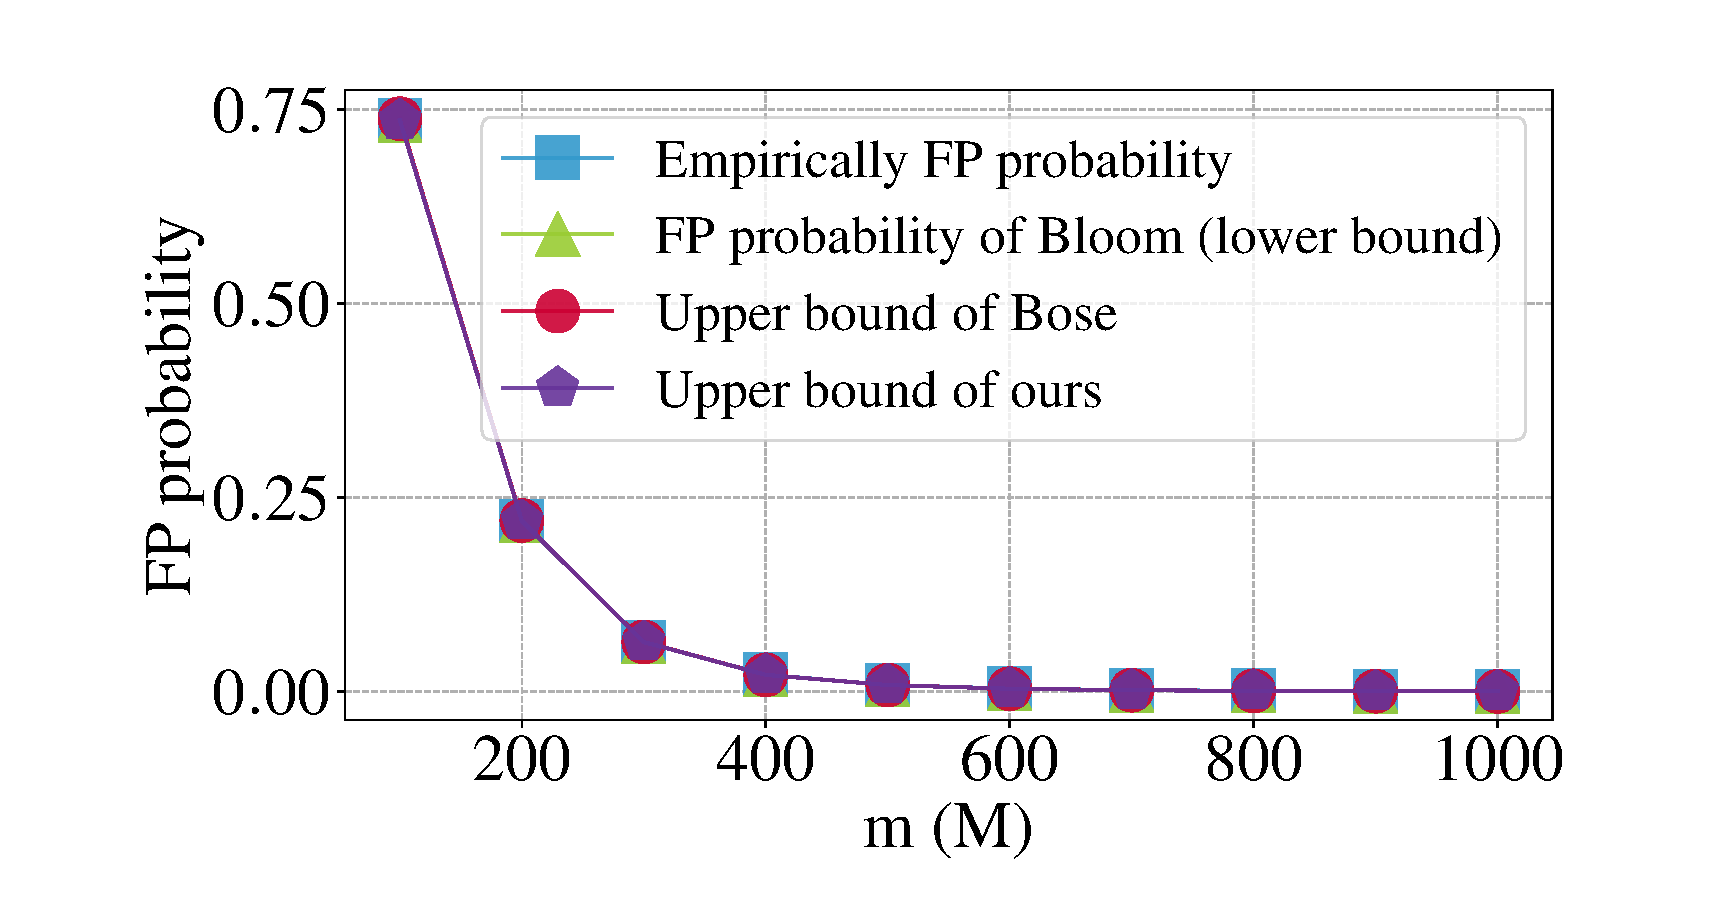
\includegraphics[width=0.90\textwidth, height=1.125in]{upbound_m}}
			\vspace{-0.02in}
		\postfig\precaption\adjustfigs
%		\vspace{-0.05in}
		\caption{FP probability vs. $m$ for $n = 50$M and $k = 6$.}
		\label{upbound_m}\postcaption
	\end{minipage}
	%
	\begin{minipage}[t]{0.32\textwidth}{
			\prefig
			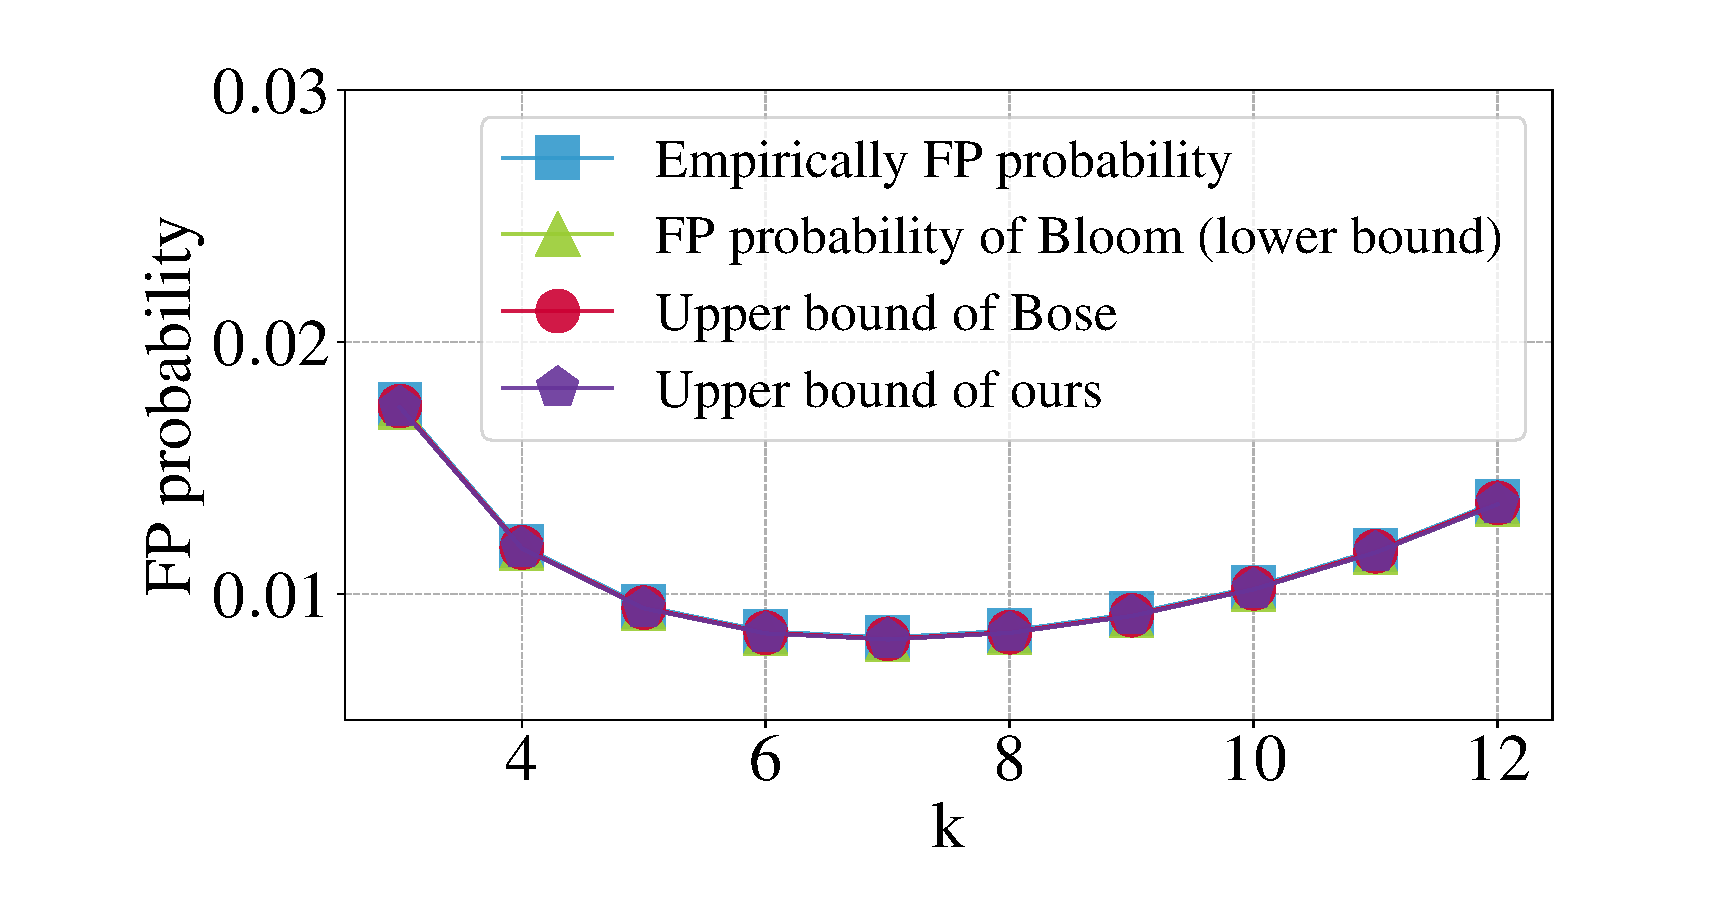
\includegraphics[width=0.90\textwidth, height=1.125in]{upbound_k}}
		\postfig\precaption\adjustfigs
%		\vspace{-0.05in}
		\caption{FP probability vs. $k$ for $n = 50$M and $m = 500$M.}
		\label{upbound_k}\postcaption
	\end{minipage}
	%
%	\vspace{-0.02in}
\end{figure*}

\begin{figure*}[t!]
	\vspace{0.1in}
	\centering
	%
	\begin{minipage}[t]{0.32\textwidth}{
			\prefig
			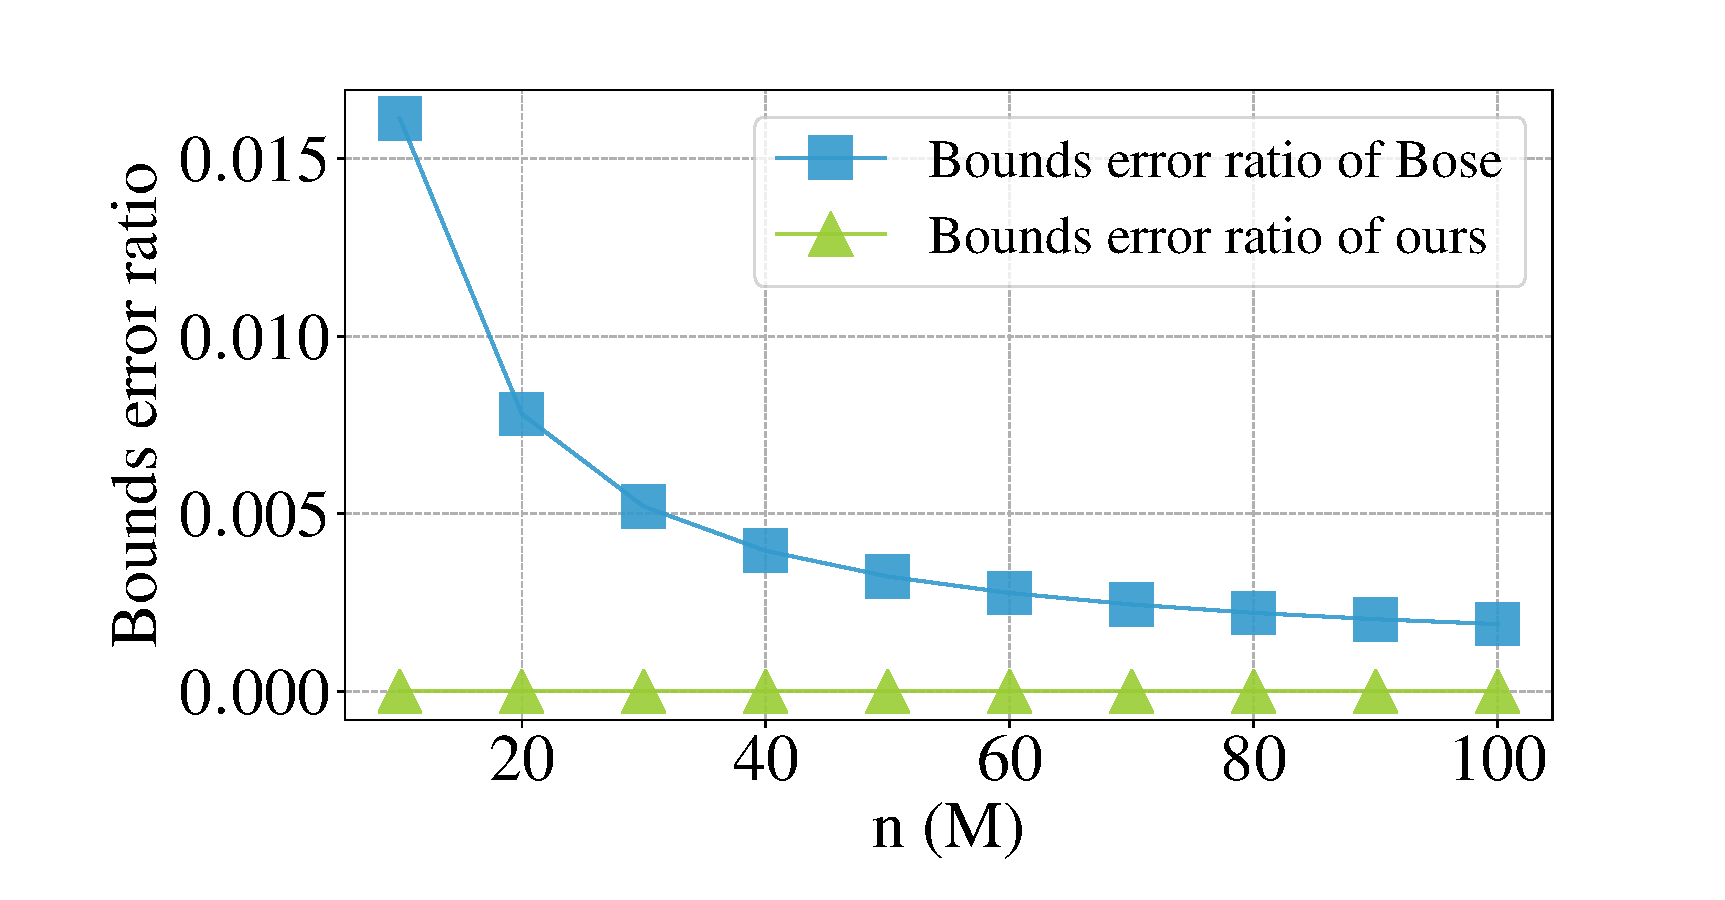
\includegraphics[width=0.90\textwidth, height=1.125in]{upbound_error_ratio_n}}
		\postfig\precaption\adjustfigs
%		\vspace{-0.05in}
		\caption{Bounds error ratio vs. $n$ for $m = 500$M and $k = 6$.}
		\label{upbound_error_ratio_n}\postcaption
	\end{minipage}
	%
	\begin{minipage}[t]{0.32\textwidth}{
			\prefig
			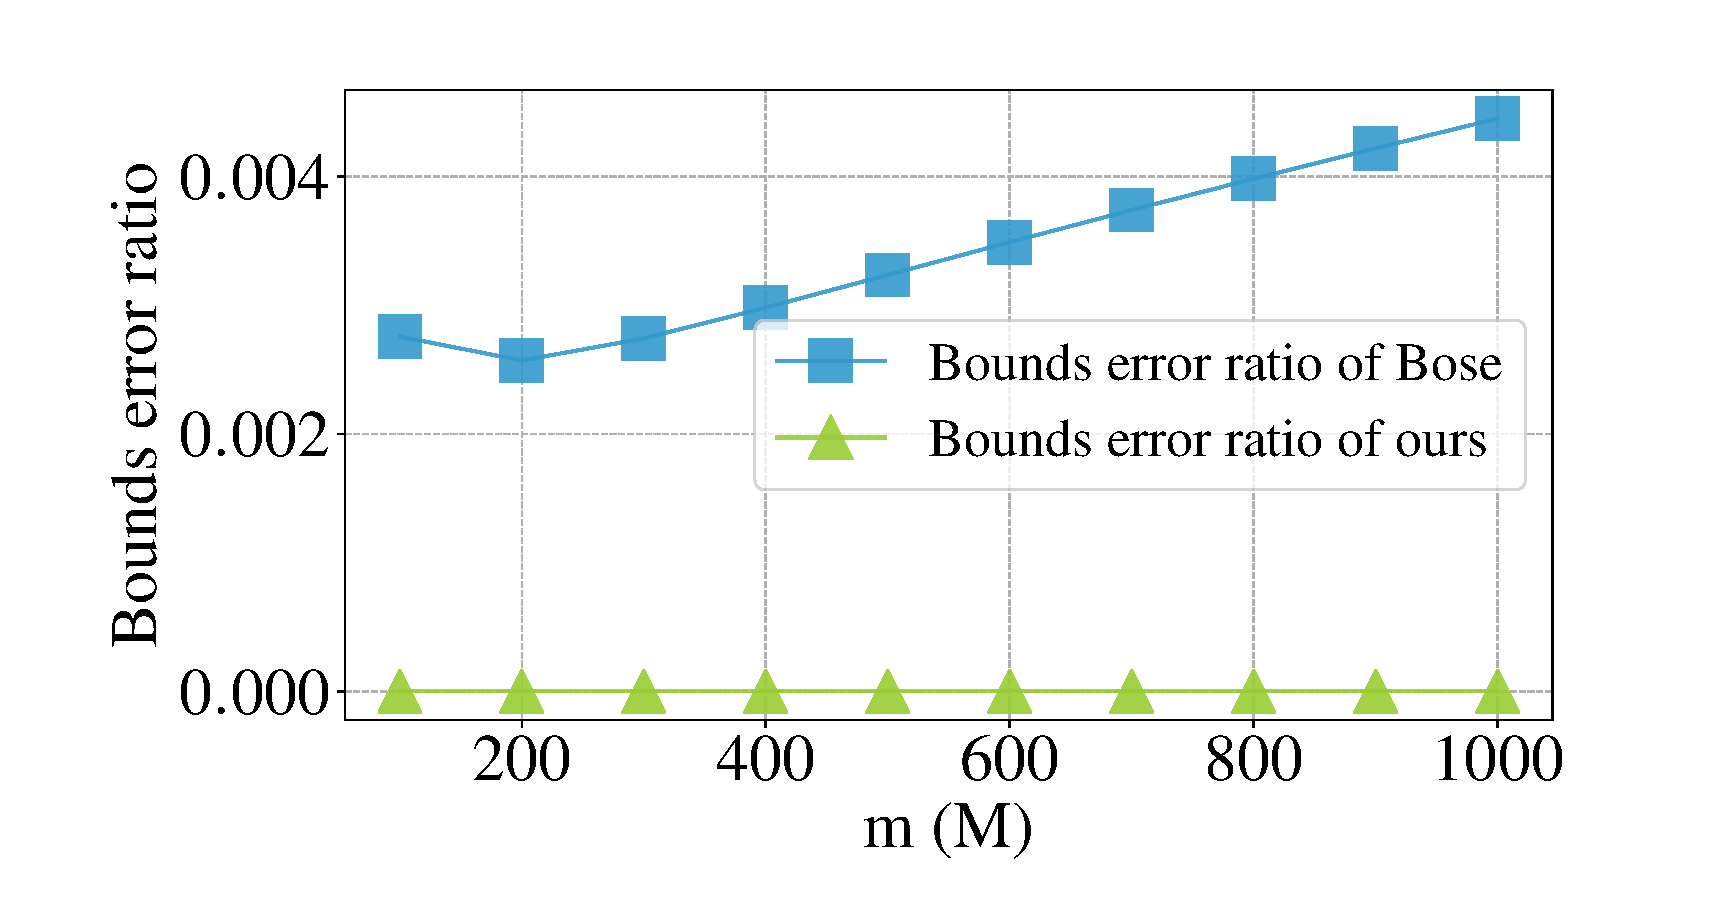
\includegraphics[width=0.90\textwidth, height=1.125in]{upbound_error_ratio_m}}
		\postfig\precaption\adjustfigs
%		\vspace{-0.05in}
		\caption{Bounds error ratio vs. $m$ for $n = 50$M and $k = 6$.}
		\label{upbound_error_ratio_m}\postcaption
	\end{minipage}
	%
	\begin{minipage}[t]{0.32\textwidth}{
			\prefig
			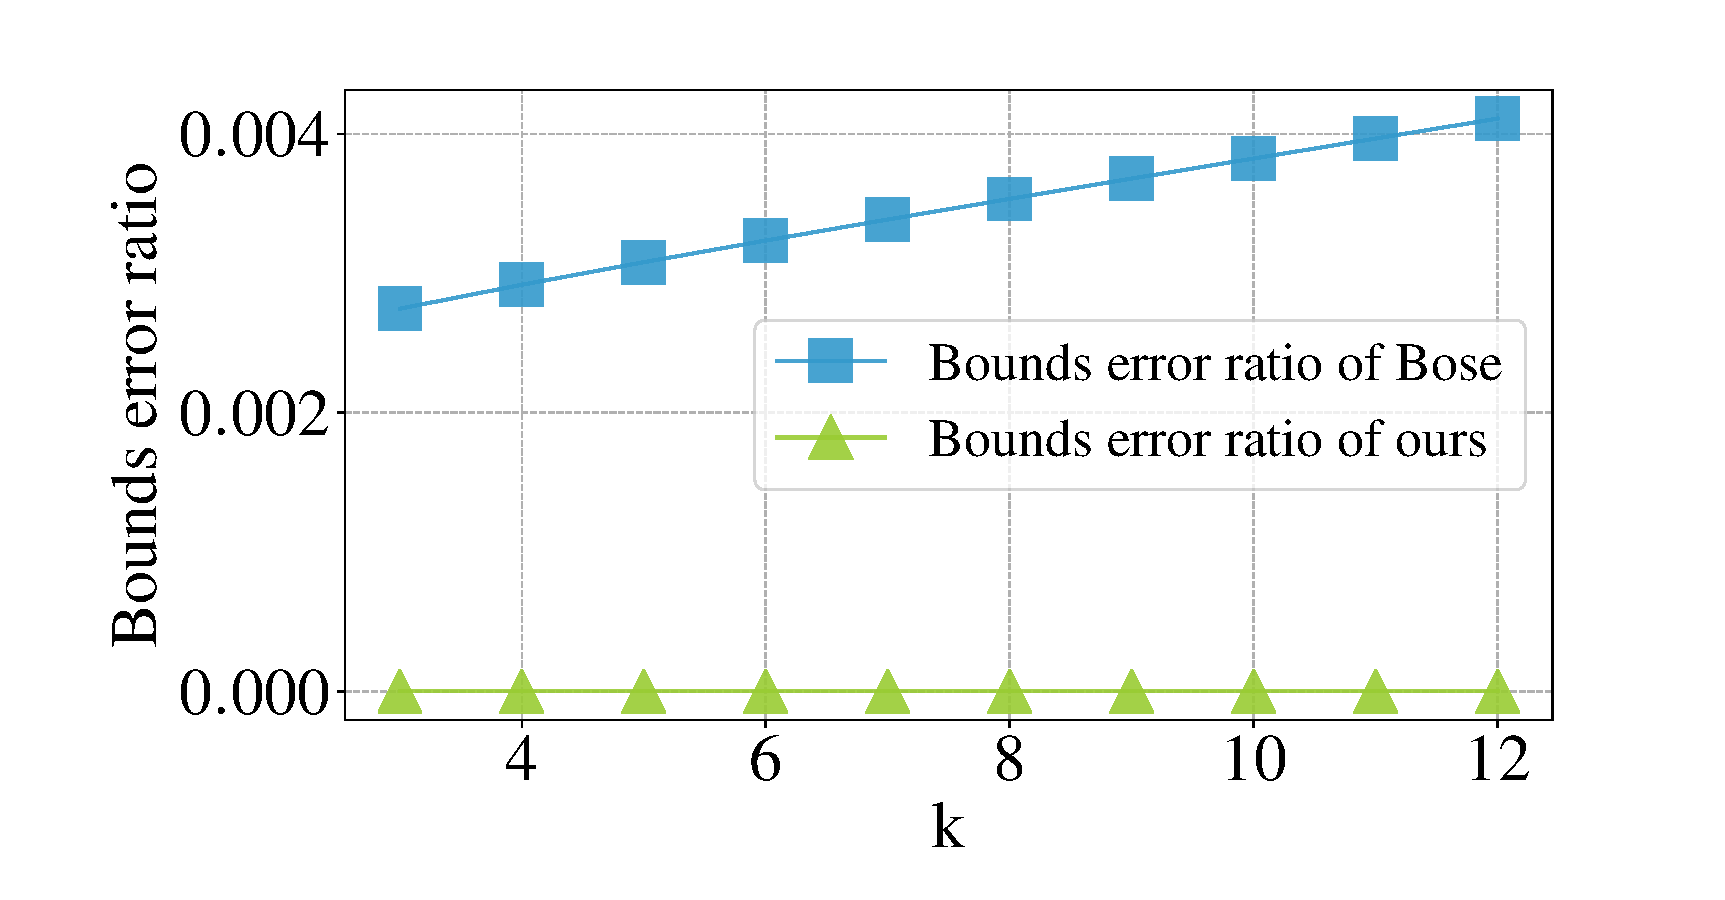
\includegraphics[width=0.90\textwidth, height=1.125in]{upbound_error_ratio_k}}
		\postfig\precaption\adjustfigs
%		\vspace{-0.05in}
		\caption{Bounds error ratio vs. $k$ for $n = 50$M and $m = 500$M.}
		\label{upbound_error_ratio_k}\postcaption
	\end{minipage}
	%
%	\vspace{-0.02in}
\end{figure*}

\begin{figure*}[t!]
	\vspace{0.1in}
	\centering
	%
	\begin{minipage}[t]{0.32\textwidth}{
			\prefig
			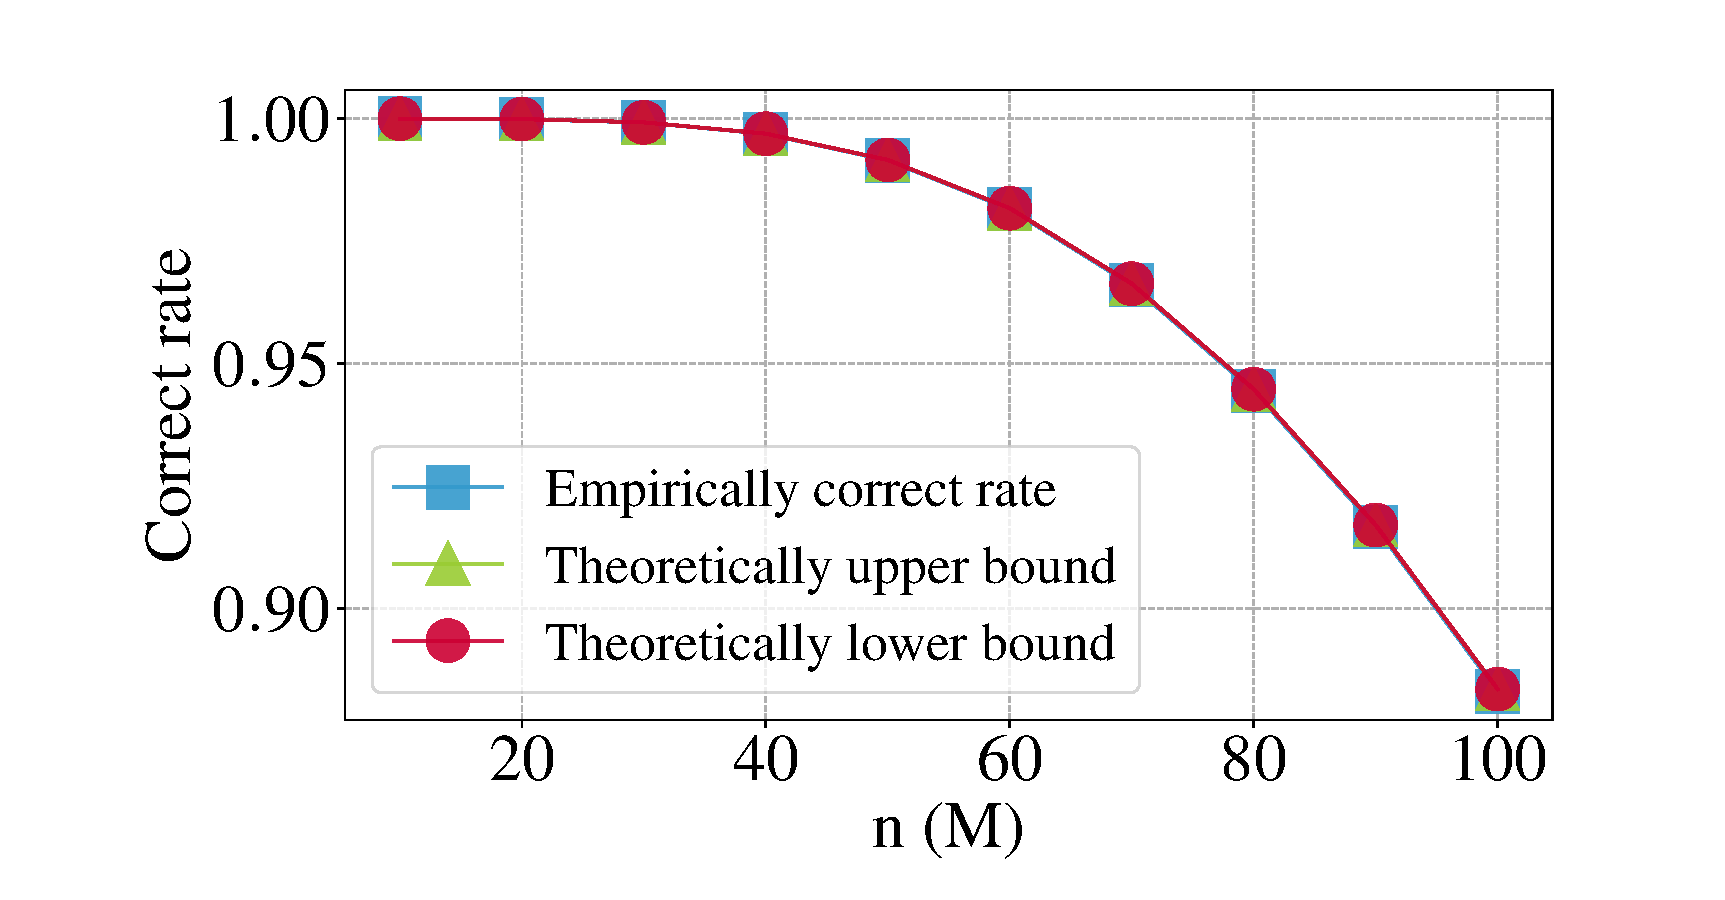
\includegraphics[width=0.90\textwidth, height=1.125in]{cr_n}}
		\postfig\precaption\adjustfigs
%		\vspace{-0.05in}
		\caption{Correct rate vs. $n$ for $m = 500$M and $k = 6$.}
		\label{cr_n}\postcaption
	\end{minipage}
	%
	\begin{minipage}[t]{0.32\textwidth}{
			\prefig
			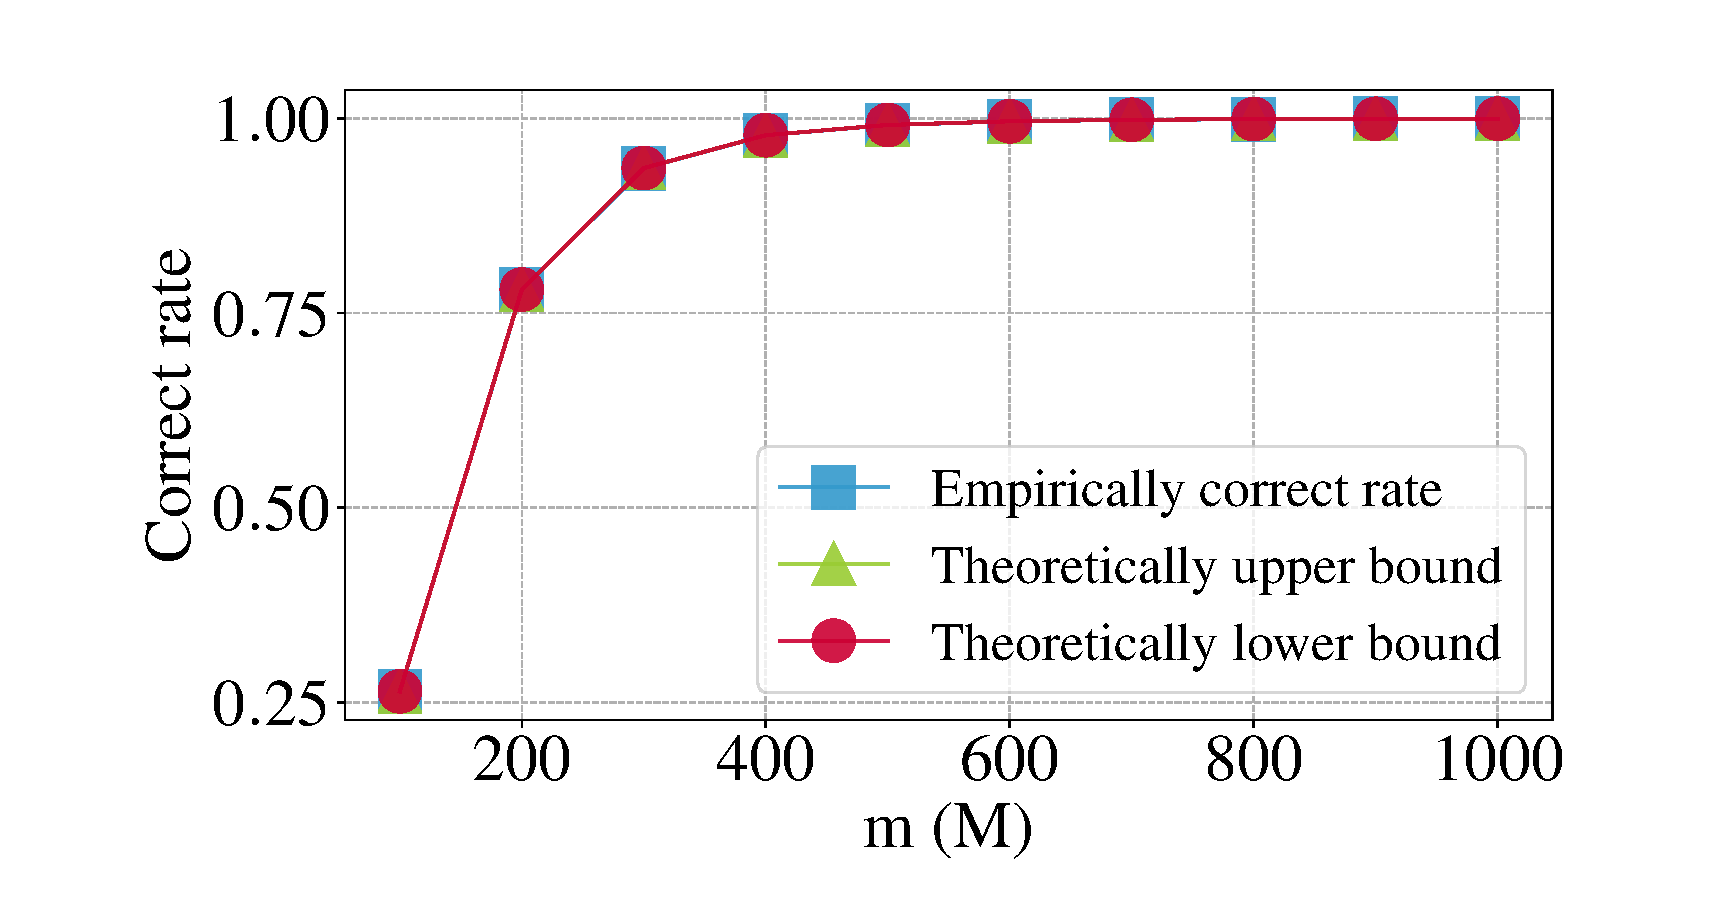
\includegraphics[width=0.90\textwidth, height=1.125in]{cr_m}}
		\postfig\precaption\adjustfigs
%		\vspace{-0.05in}
		\caption{Correct rate vs. $m$ for $n = 50$M and $k = 6$.}
		\label{cr_m}\postcaption
	\end{minipage}
	%
	\begin{minipage}[t]{0.32\textwidth}{
			\prefig
			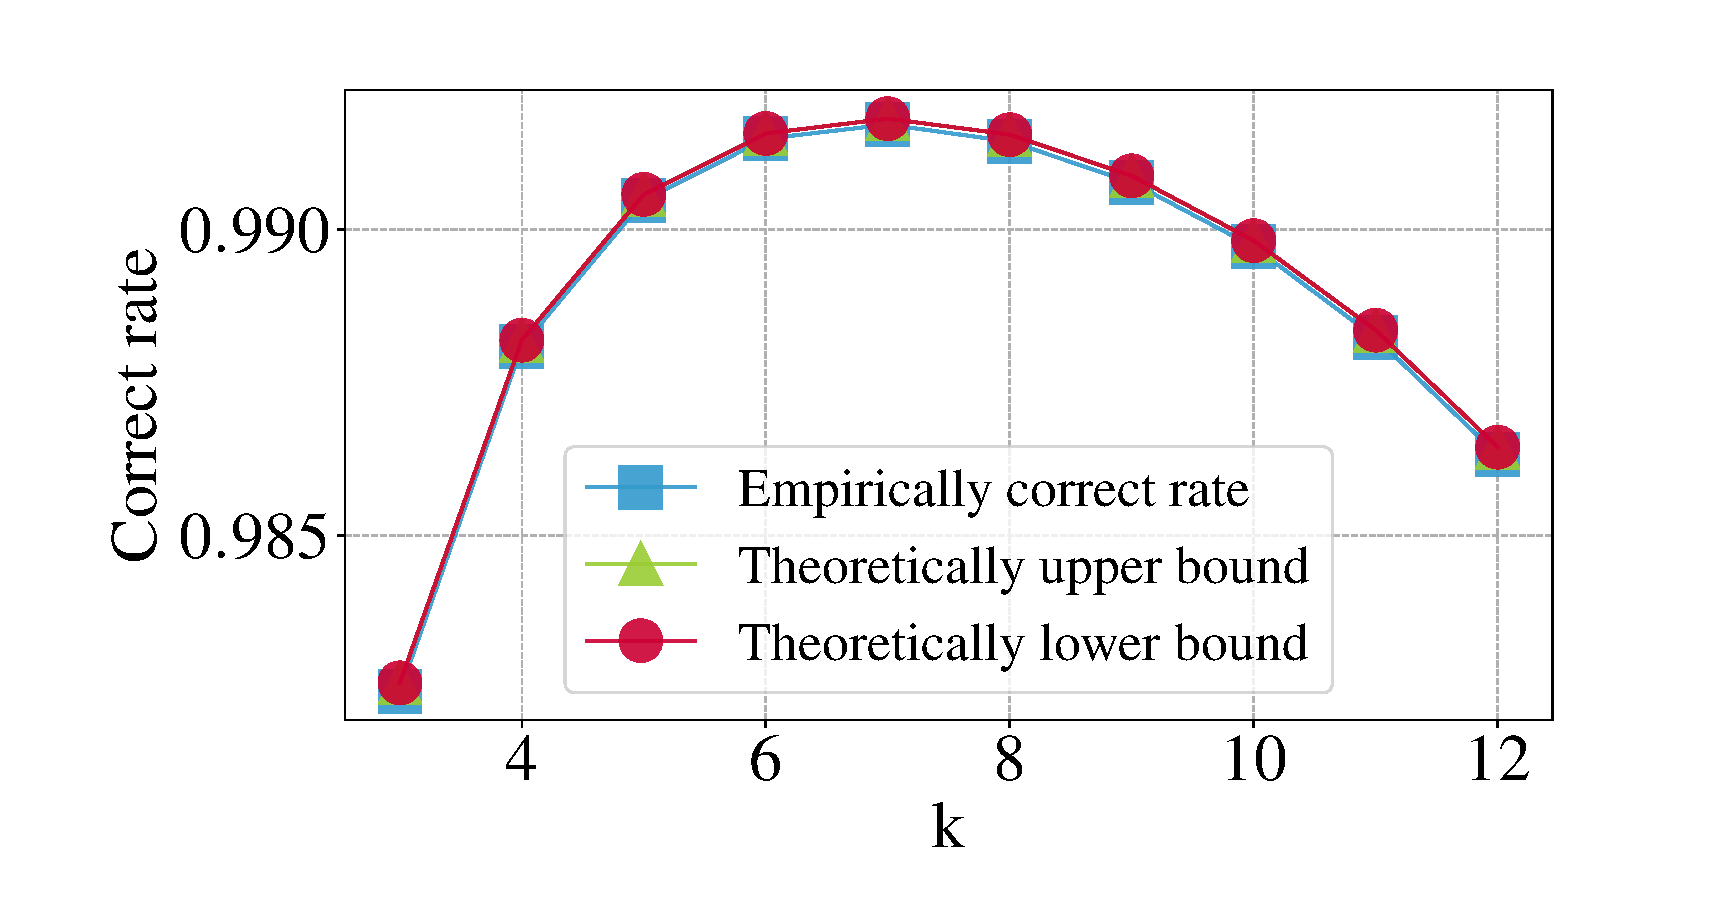
\includegraphics[width=0.90\textwidth, height=1.125in]{cr_k}}
		\postfig\precaption\adjustfigs
%		\vspace{-0.05in}
		\caption{Correct rate vs. $k$ for $n = 50$M and $m = 500$M.}
		\label{cr_k}\postcaption
	\end{minipage}
	%
%	\vspace{-0.03in}
\end{figure*}

\subsubsection{Upper Bound vs. $n$}

Figure \ref{upbound_n} plots the empirical results, Bloom's theoretical results, Bose's upper bounds, and our upper bounds of FP probability with different $n$ increasing from 10M to 100M with a step of 10M for $m = 500$M and $k = 6$. 
\textit{Our results show that our upper bounds of FP probability follows the empirical FP probability very well, regardless of the values of $n$.} 
We find that all above four results almost coincide with each other, which demonstrates the tightness of bounds in Eq. \ref{fBound} and \ref{bounds}. 

To compare upper bound of Bose and ours more intuitively, in Figure \ref{upbound_error_ratio_n}, we plot the bounds error ratios $\beta$, defined as $\beta=\frac{upper\ bound - lower\ bound}{lower\ bound}$, of these two upper bounds with different $n$ increasing from 10M to 100M with a step of 10M for $m = 500$M and $k = 6$. 
\textit{Our results show that the bounds error ratio of our upper bound is $26821.2\sim125492.5$ lower than that of Bose's upper bound. }
We find that our upper bound almost coincides with the lower bound, which demonstrates the superiority of our upper bound. 







%\begin{figure}[htbp]
%	\prefig
%	\centering
%	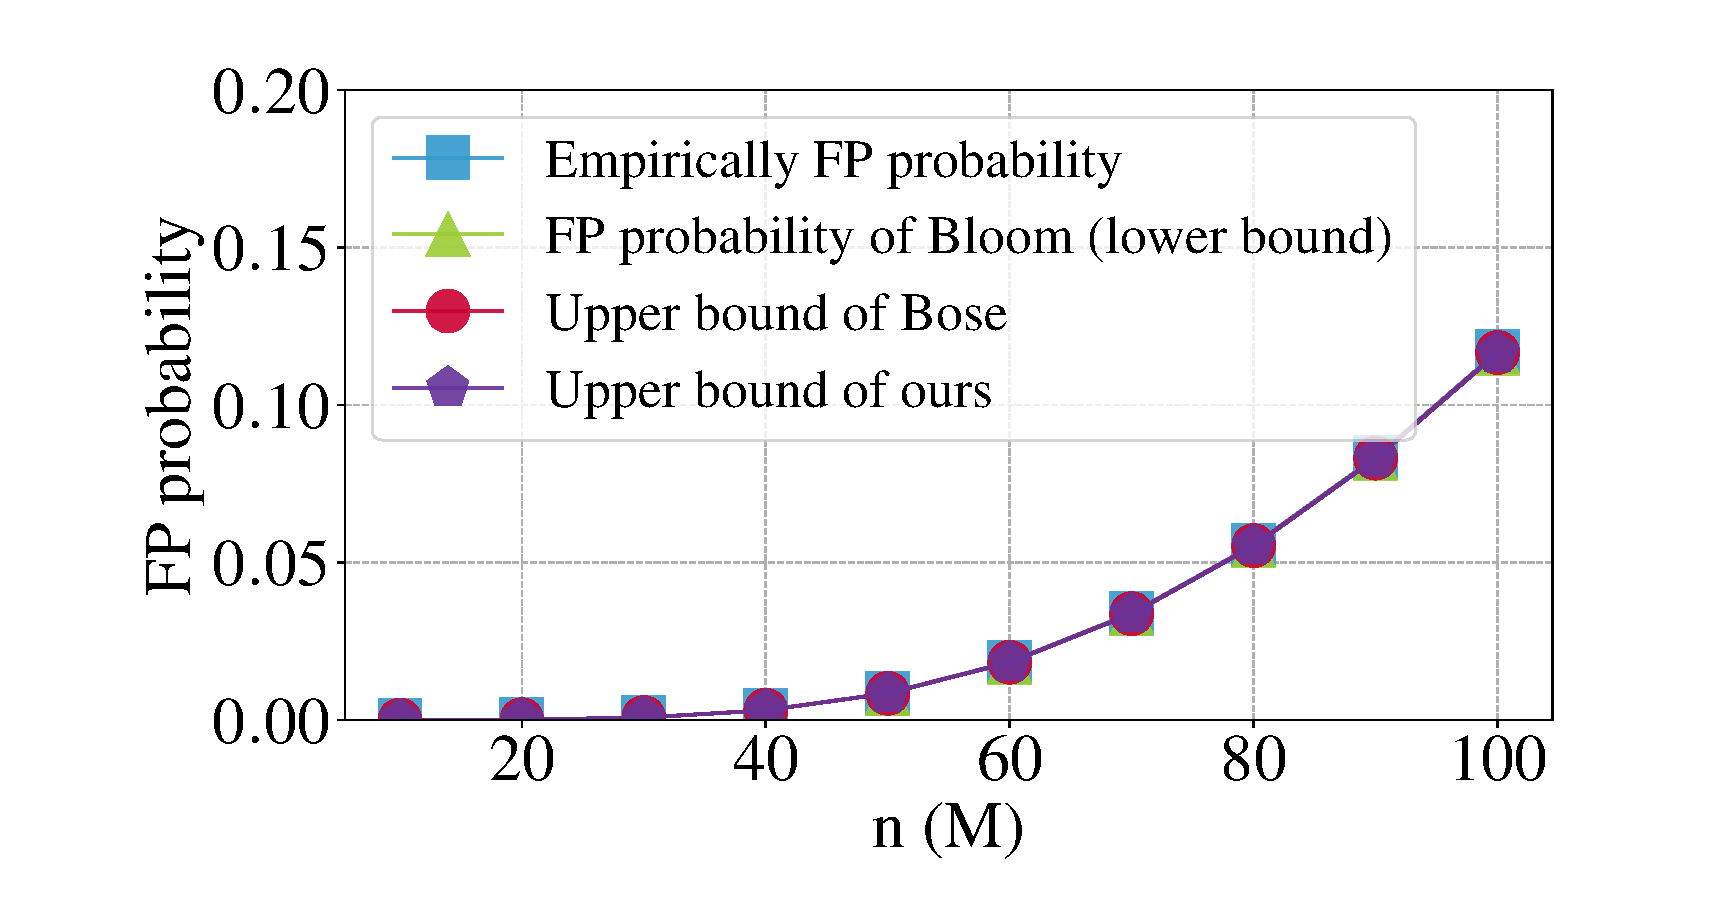
\includegraphics[width=\figwidthdraw]{upbound_n}
%	\postfig\precaption
%	\caption{FP probability vs. $n$ for $m = 500$M and $k = 6$.}
%	\label{upbound_n}
%	\postcaption
%\end{figure}
%
%
%\begin{figure}[htbp]
%	\prefig
%	\centering
%	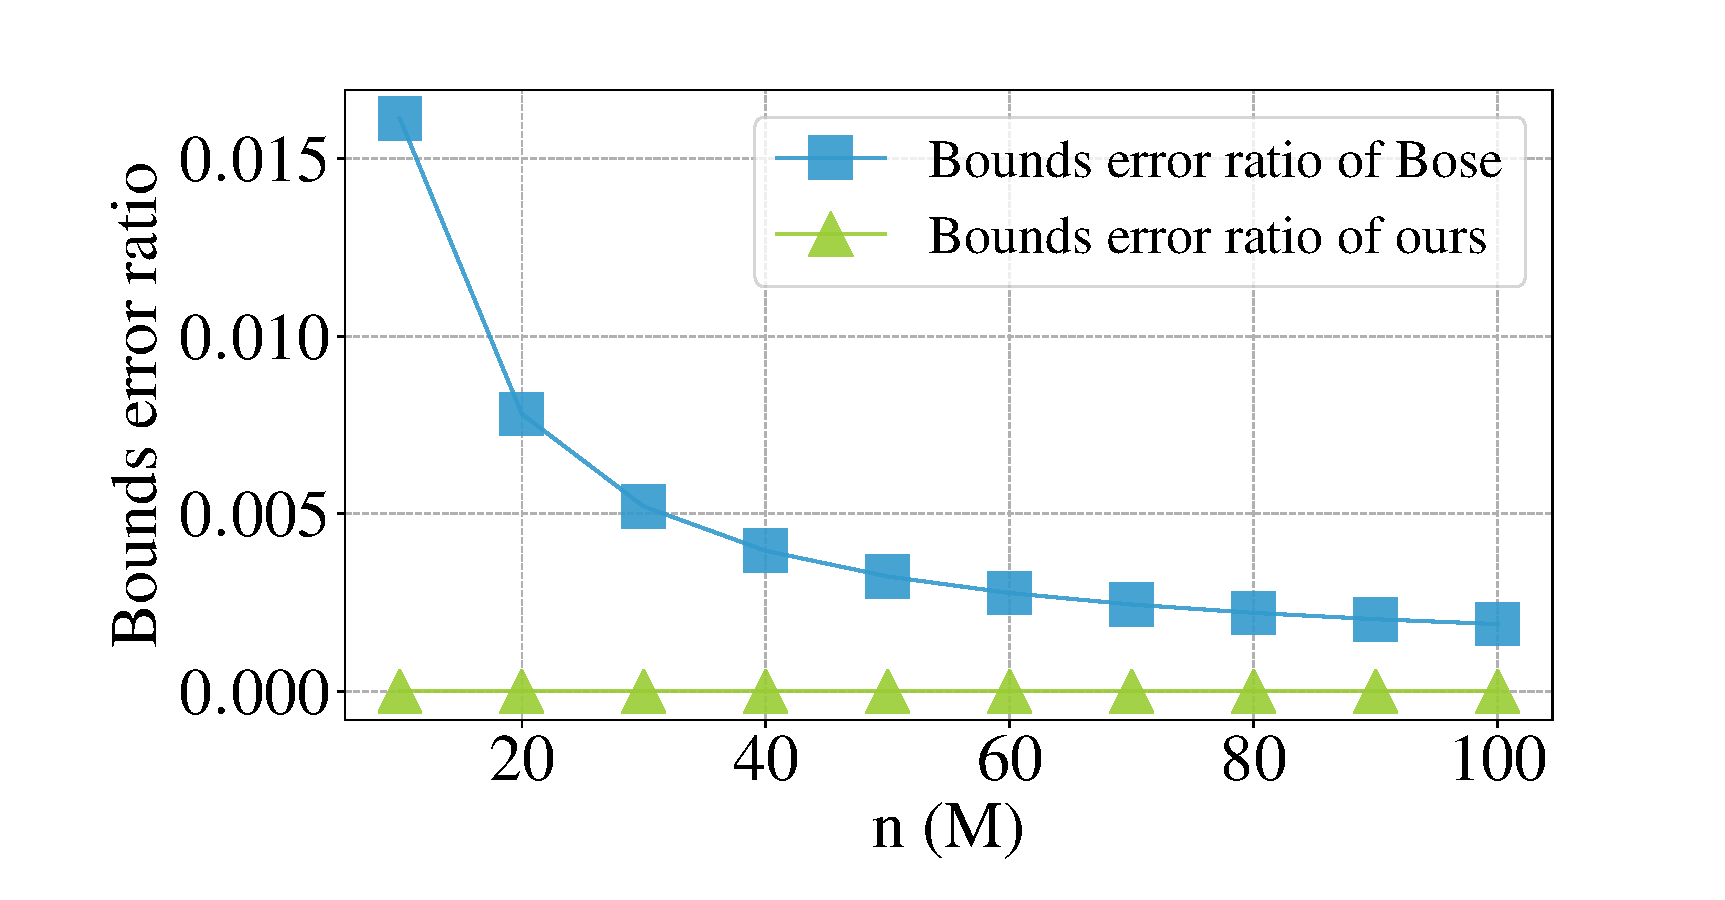
\includegraphics[width=\figwidthdraw]{upbound_error_ratio_n}
%	\postfig\precaption
%	\caption{Bounds error ratio vs. $n$ for $m = 500$M and $k = 6$.}
%	\label{upbound_error_ratio_n}
%	\postcaption
%\end{figure}


\subsubsection{Upper Bound vs. $m$}

Figure \ref{upbound_m} plots the empirical results, Bloom's theoretical results, Bose's upper bounds, and our upper bounds of FP probability with different $m$ increasing from 100M to 1000M with a step of 100M for $n = 50$M and $k = 6$. 
\textit{Our results show that our upper bounds of FP probability follows the empirical FP probability very well, regardless of the values of $m$.} 
%We find that all above four results almost coincide with each other, which demonstrates the tightness of bounds in Eq. \ref{fBound} and \ref{bounds}. 

Figure \ref{upbound_error_ratio_m} plots the bounds error ratios of these two upper bounds with different $m$ increasing from 100M to 1000M with a step of 100M for $n = 50$M and $k = 6$. 
\textit{Our results show that the bounds error ratio of our upper bound is $21885.4\sim150182.6$ lower than that of Bose's upper bound. }
We find that our upper bound almost coincides with the lower bound, regardless of the values of $m$. 


%\begin{figure}[htbp]
%	\prefig
%	\centering
%	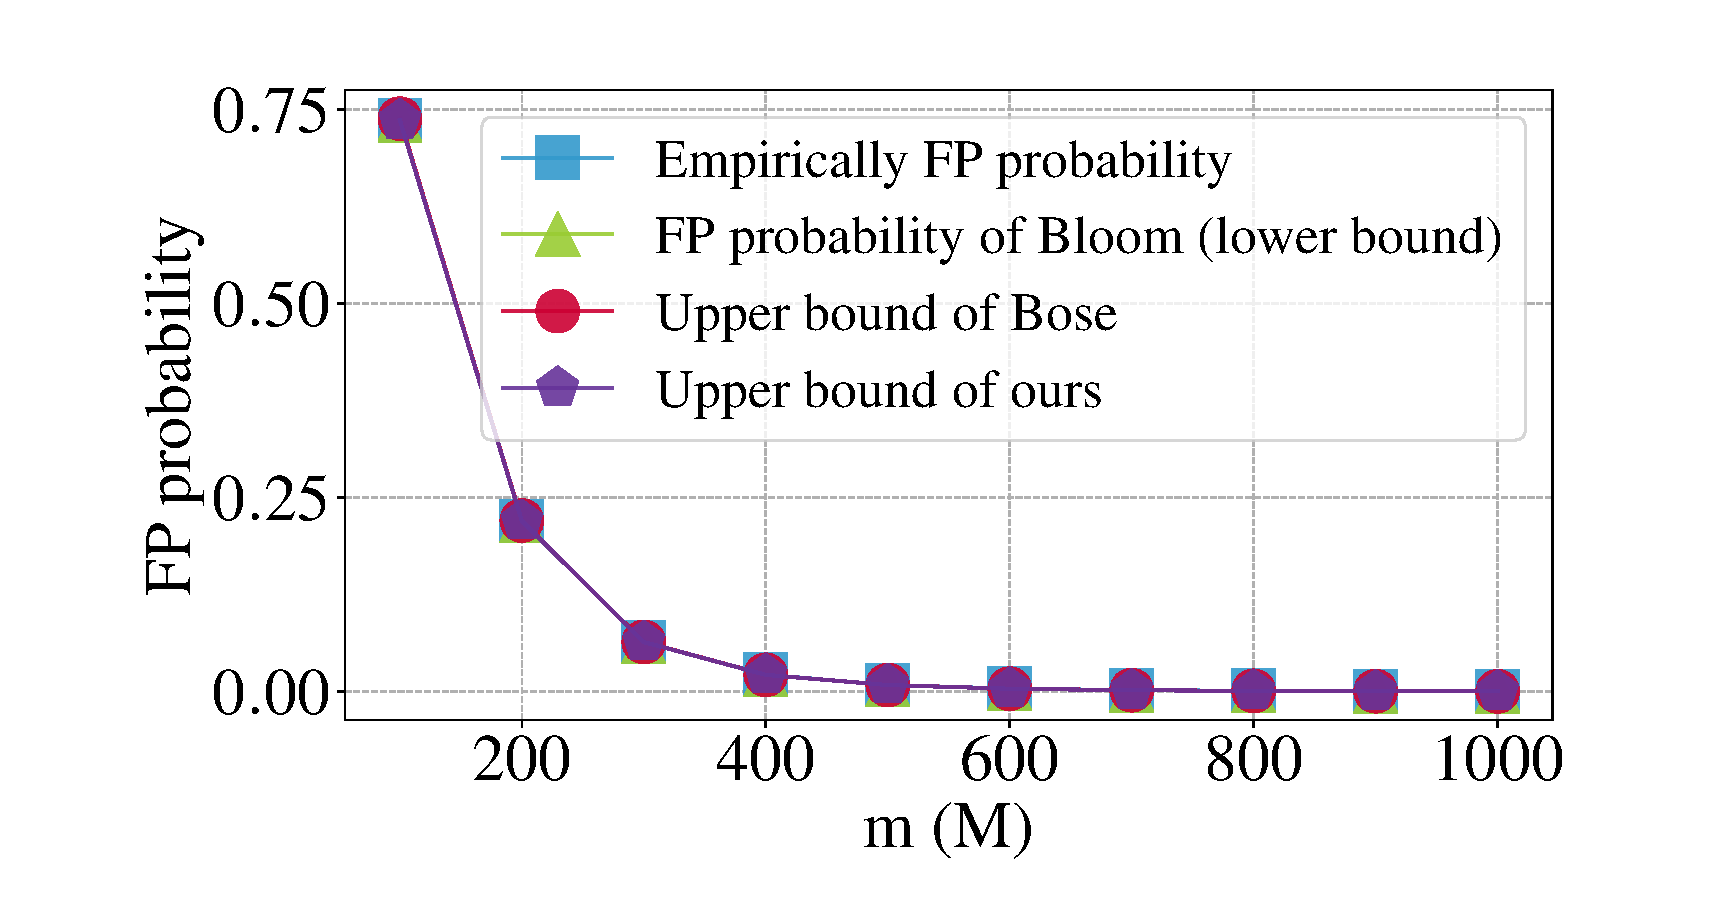
\includegraphics[width=\figwidthdraw]{upbound_m}
%	\postfig\precaption
%	\caption{FP probability vs. $m$ for $n = 50$M and $k = 6$.}
%	\label{upbound_m}
%	\postcaption
%\end{figure}
%
%
%\begin{figure}[htbp]
%	\prefig
%	\centering
%	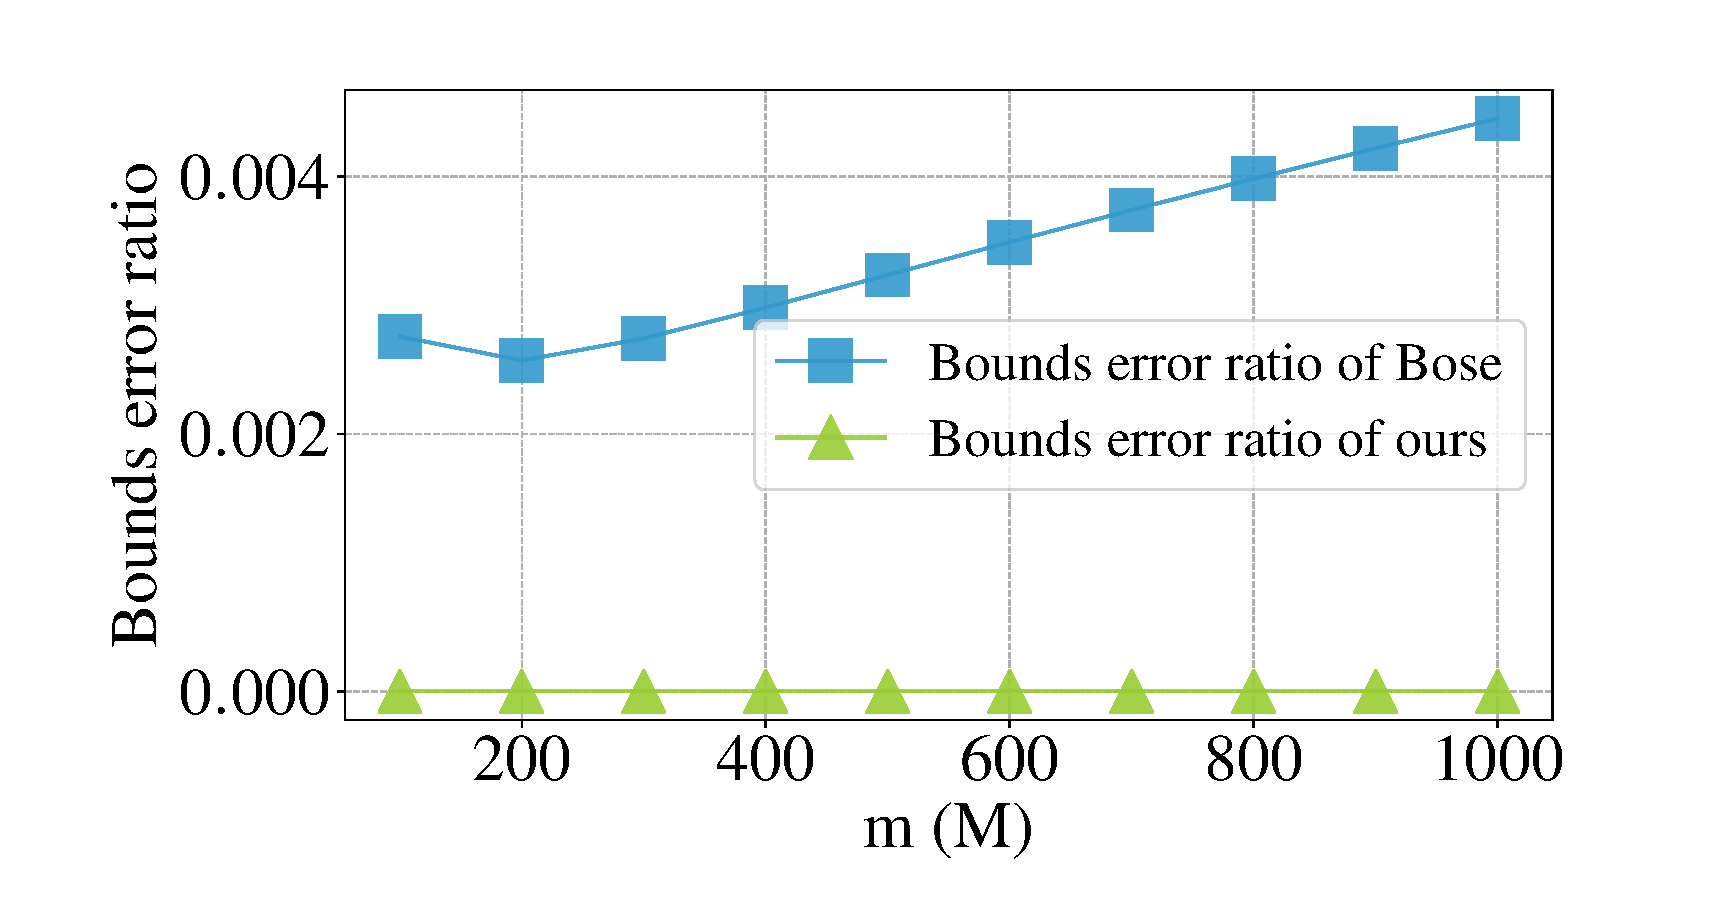
\includegraphics[width=\figwidthdraw]{upbound_error_ratio_m}
%	\postfig\precaption
%	\caption{Bounds error ratio vs. $m$ for $n = 50$M and $k = 6$.}
%	\label{upbound_error_ratio_m}
%	\postcaption
%\end{figure}


\subsubsection{Upper Bound vs. $k$}

Figure \ref{upbound_k} plots the empirical results, Bloom's theoretical results, Bose's upper bounds, and our upper bounds of FP probability with different $k$ increasing from 3 to 12 with a step of 1 for $n = 50$M and $m = 500$M. 
\textit{Our results show that our upper bounds of FP probability follows the empirical FP probability very well, regardless of the values of $k$.} 
%We find that all above four results almost coincide with each other, which demonstrates the tightness of bounds in Eq. \ref{fBound} and \ref{bounds}. 

Figure \ref{upbound_error_ratio_k} plots the bounds error ratios of these two upper bounds with different $k$ increasing from 3 to 12 with a step of 1 for $n = 50$M and $m = 500$M. 
\textit{Our results show that the bounds error ratio of our upper bound is $39483.8\sim64668.5$ lower than that of Bose's upper bound. }
%We find that our upper bound almost coincides with the lower bound, which demonstrates the superiority of our upper bound. 

%\begin{figure}[htbp]
%	\prefig
%	\centering
%	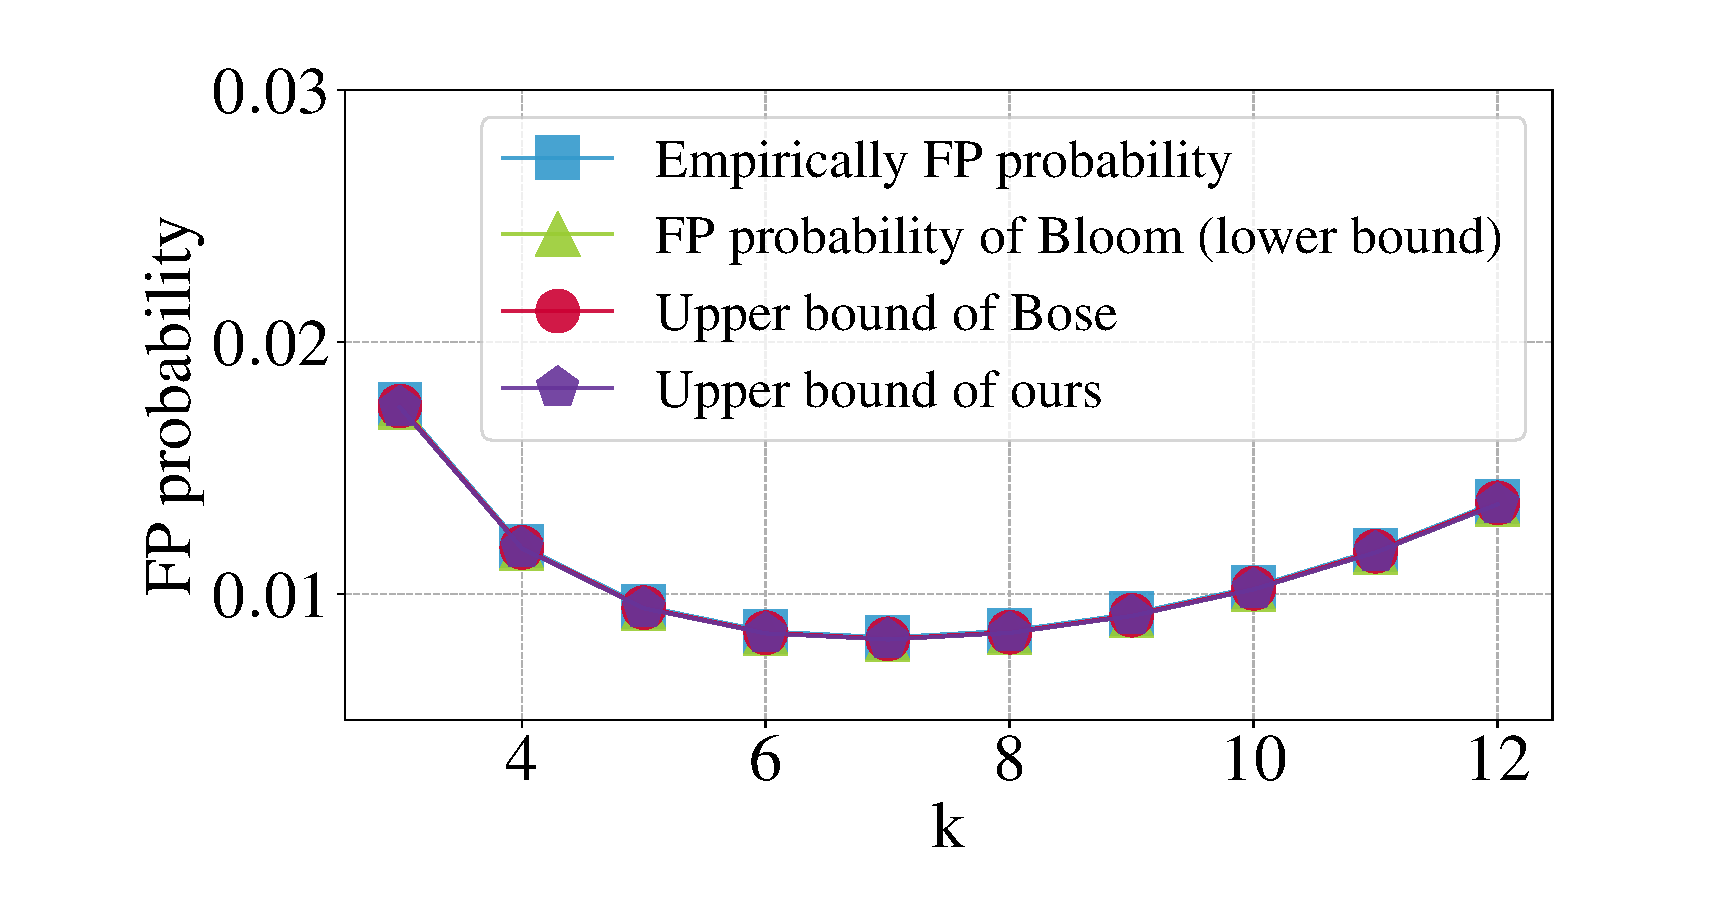
\includegraphics[width=\figwidthdraw]{upbound_k}
%	\postfig\precaption
%	\caption{FP probability vs. $k$ for $n = 50$M and $m = 500$M.}
%	\label{upbound_k}
%	\postcaption
%\end{figure}
%
%
%\begin{figure}[htbp]
%	\prefig
%	\centering
%	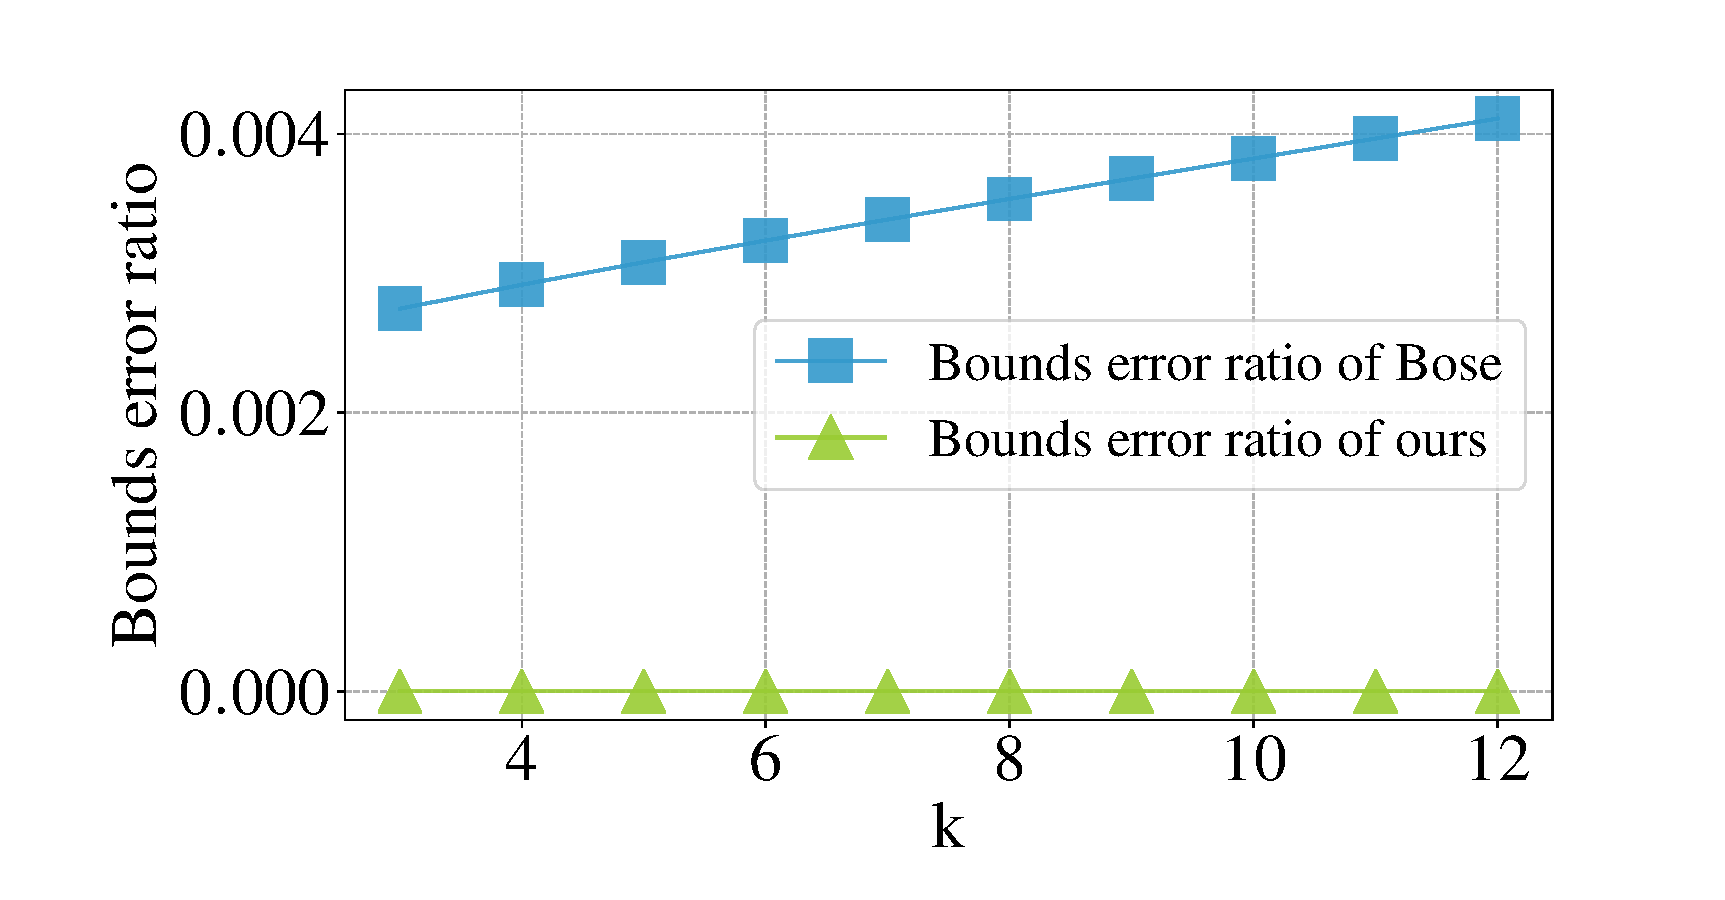
\includegraphics[width=\figwidthdraw]{upbound_error_ratio_k}
%	\postfig\precaption
%	\caption{Bounds error ratio vs. $k$ for $n = 50$M and $m = 500$M.}
%	\label{upbound_error_ratio_k}
%	\postcaption
%\end{figure}

\vspace{-0.05in}
\subsection{$\mathcal{C}_r$ Formula Validation}
\vspace{-0.02in}
Figure \ref{cr_n}, \ref{cr_m}, and \ref{cr_k} plot the correct rates of CFBs with different values of $n$, $m$, and $k$, respectively. 
\textit{Our results show that our lower and upper bounds of the correct rate of CBFs follow the empirical correct rates very well, regardless of the values of $n$, $m$, and $k$.}

 
%
%\subsubsection{Correct Rate vs. $n$}
%
%\subsubsection{Correct Rate vs. $m$}
%
%\subsubsection{Correct Rate vs. $k$}
